\chapter{Method}
\label{ch:method}

\section{The dataset}
The dataset consists of manually labeled recorded movies of 20 different people
performing the complete sequence of hand poses.

Usually the 12 Curwen solfege hand symbols are performed in front of the torso
as shown in Figure~\ref{fig:hands_normal}. To increase the number of hand poses
to be recogniced, all 12 Curwen are also performed mirrored next to the body of
the recorded subject, see Figure~\ref{fig:hands_mirrored}. Additionally four
extra hand symbols have been added that are not part of the Curwen sequence, see
Figure~\ref{fig:hands_extra}. These last four symbols are performed next to the
head.


%\renewcommand{\thesubfigure}{\thefigure.\arabic{subfigure}} 
\begin{figure}[htbp]
\begin{center}
\subfloat[Do]{\label{fig:hand_0}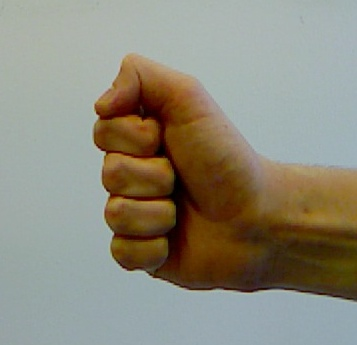
\includegraphics[width=0.2\linewidth,height=0.15\linewidth]{figures/examples/0.jpg}}
\hspace{0.03\linewidth}
\subfloat[Di]{\label{fig:hand_1}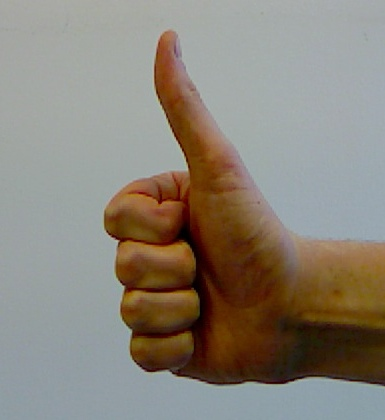
\includegraphics[width=0.2\linewidth,height=0.15\linewidth]{figures/examples/1.jpg}}
\hspace{0.03\linewidth}
\subfloat[Re]{\label{fig:hand_2}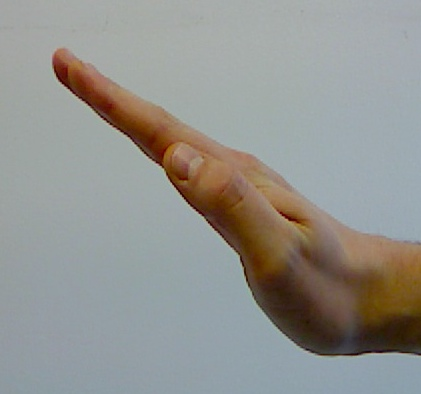
\includegraphics[width=0.2\linewidth,height=0.15\linewidth]{figures/examples/2.jpg}}
\hspace{0.03\linewidth}
\subfloat[Ri]{\label{fig:hand_3}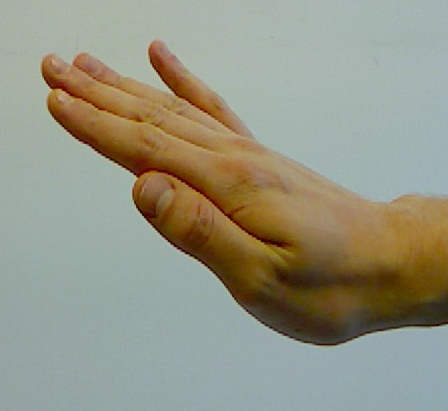
\includegraphics[width=0.2\linewidth,height=0.15\linewidth]{figures/examples/3.jpg}}
\hspace{0.03\linewidth}
\subfloat[Mi]{\label{fig:hand_4}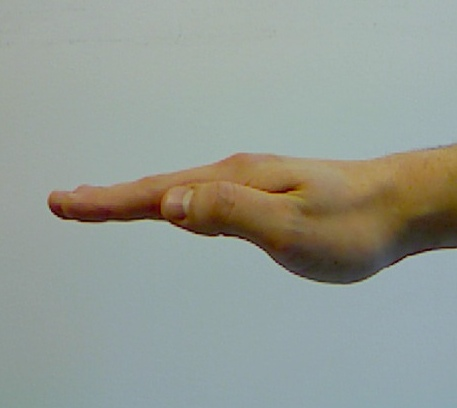
\includegraphics[width=0.2\linewidth,height=0.15\linewidth]{figures/examples/4.jpg}}
\hspace{0.03\linewidth}
\subfloat[Fa]{\label{fig:hand_5}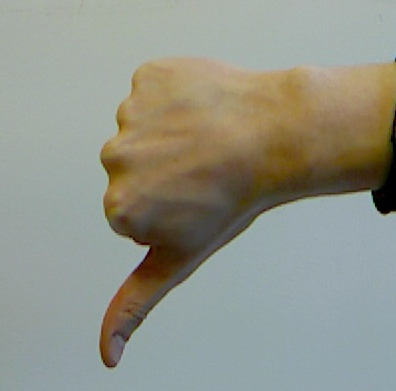
\includegraphics[width=0.2\linewidth,height=0.15\linewidth]{figures/examples/5.jpg}}
\hspace{0.03\linewidth}
\subfloat[Fi]{\label{fig:hand_6}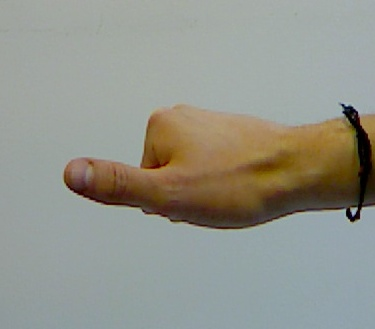
\includegraphics[width=0.2\linewidth,height=0.15\linewidth]{figures/examples/6.jpg}}
\hspace{0.03\linewidth}
\subfloat[Sol]{\label{fig:hand_7}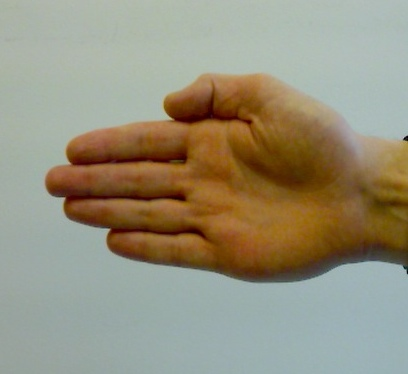
\includegraphics[width=0.2\linewidth,height=0.15\linewidth]{figures/examples/7.jpg}}
\hspace{0.03\linewidth}
\subfloat[Si]{\label{fig:hand_8}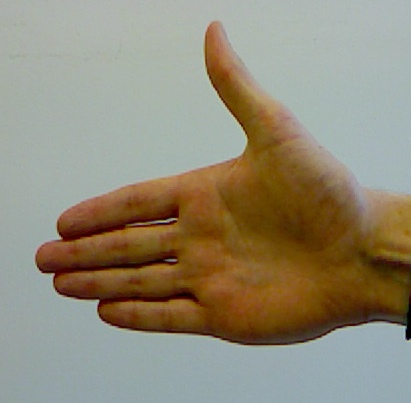
\includegraphics[width=0.2\linewidth,height=0.15\linewidth]{figures/examples/8.jpg}}
\hspace{0.03\linewidth}
\subfloat[La]{\label{fig:hand_9}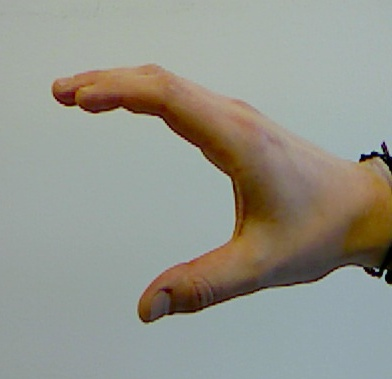
\includegraphics[width=0.2\linewidth,height=0.15\linewidth]{figures/examples/9.jpg}}
\hspace{0.03\linewidth}
\subfloat[Li]{\label{fig:hand_10}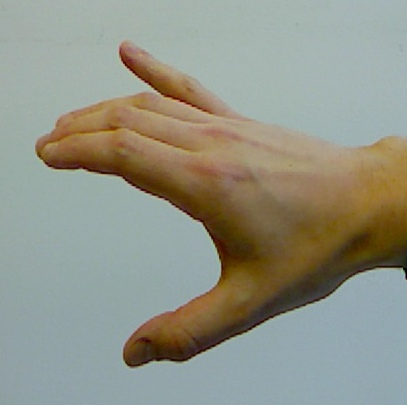
\includegraphics[width=0.2\linewidth,height=0.15\linewidth]{figures/examples/10.jpg}}
\hspace{0.03\linewidth}
\subfloat[Ti]{\label{fig:hand_11}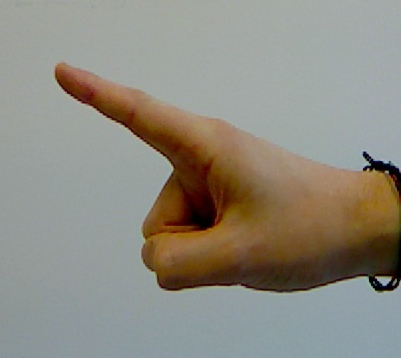
\includegraphics[width=0.2\linewidth,height=0.15\linewidth]{figures/examples/11.jpg}}
\end{center}
\caption{All mirrored Curwen hand poses}
\label{fig:hands_mirrored}
\end{figure}

\begin{figure}[htbp]
\begin{center}
\subfloat[Do]{\label{fig:hand_12}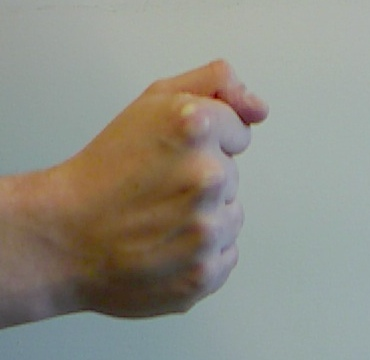
\includegraphics[width=0.2\linewidth,height=0.15\linewidth]{figures/examples/12.jpg}}
\hspace{0.03\linewidth}
\subfloat[Di]{\label{fig:hand_13}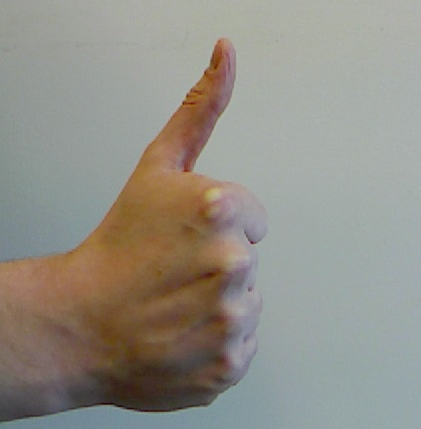
\includegraphics[width=0.2\linewidth,height=0.15\linewidth]{figures/examples/13.jpg}}
\hspace{0.03\linewidth}
\subfloat[Re]{\label{fig:hand_14}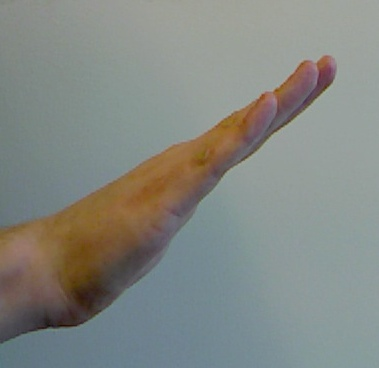
\includegraphics[width=0.2\linewidth,height=0.15\linewidth]{figures/examples/14.jpg}}
\hspace{0.03\linewidth}
\subfloat[Ri]{\label{fig:hand_15}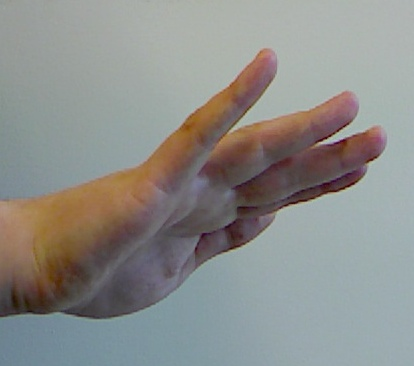
\includegraphics[width=0.2\linewidth,height=0.15\linewidth]{figures/examples/15.jpg}}
\hspace{0.03\linewidth}
\subfloat[Mi]{\label{fig:hand_16}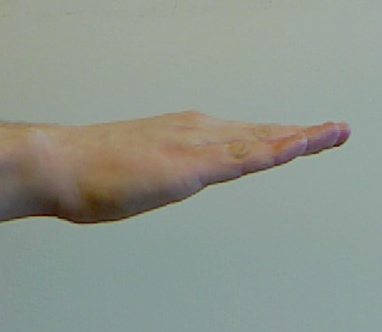
\includegraphics[width=0.2\linewidth,height=0.15\linewidth]{figures/examples/16.jpg}}
\hspace{0.03\linewidth}
\subfloat[Fa]{\label{fig:hand_17}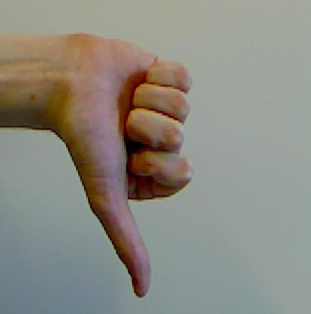
\includegraphics[width=0.2\linewidth,height=0.15\linewidth]{figures/examples/17.jpg}}
\hspace{0.03\linewidth}
\subfloat[Fi]{\label{fig:hand_18}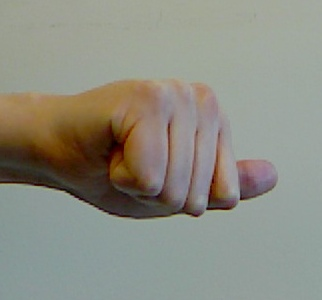
\includegraphics[width=0.2\linewidth,height=0.15\linewidth]{figures/examples/18.jpg}}
\hspace{0.03\linewidth}
\subfloat[Sol]{\label{fig:hand_19}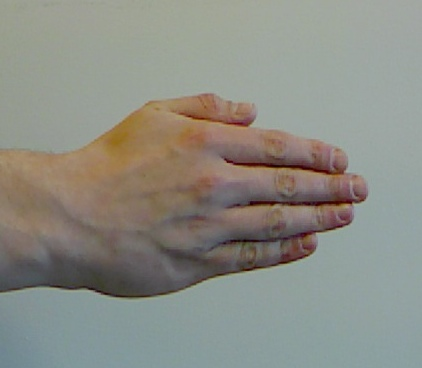
\includegraphics[width=0.2\linewidth,height=0.15\linewidth]{figures/examples/19.jpg}}
\hspace{0.03\linewidth}
\subfloat[Si]{\label{fig:hand_20}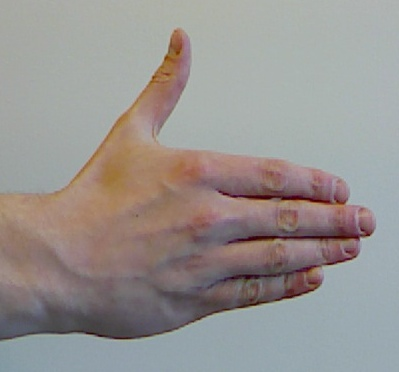
\includegraphics[width=0.2\linewidth,height=0.15\linewidth]{figures/examples/20.jpg}}
\hspace{0.03\linewidth}
\subfloat[La]{\label{fig:hand_21}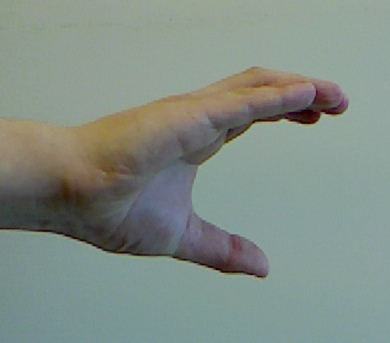
\includegraphics[width=0.2\linewidth,height=0.15\linewidth]{figures/examples/21.jpg}}
\hspace{0.03\linewidth}
\subfloat[Li]{\label{fig:hand_22}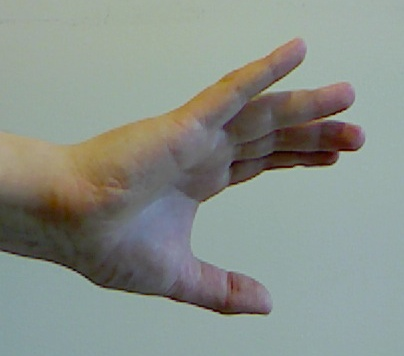
\includegraphics[width=0.2\linewidth,height=0.15\linewidth]{figures/examples/22.jpg}}
\hspace{0.03\linewidth}
\subfloat[Ti]{\label{fig:hand_23}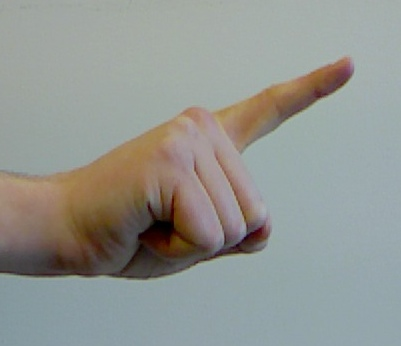
\includegraphics[width=0.2\linewidth,height=0.15\linewidth]{figures/examples/23.jpg}}
\end{center}
\caption{All Curwen hand poses}
\label{fig:hands_normal}
\end{figure}


\begin{figure}[htbp]
\begin{center}
\subfloat[Extra1]{\label{fig:hand_24}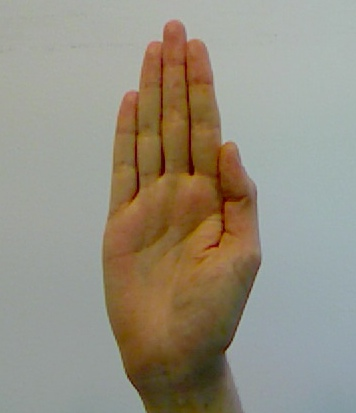
\includegraphics[width=0.2\linewidth,height=0.15\linewidth]{figures/examples/24.jpg}}
\hspace{0.03\linewidth}
\subfloat[Extra2]{\label{fig:hand_25}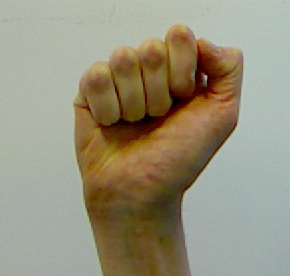
\includegraphics[width=0.2\linewidth,height=0.15\linewidth]{figures/examples/25.jpg}}
\hspace{0.03\linewidth}
\subfloat[Extra3]{\label{fig:hand_26}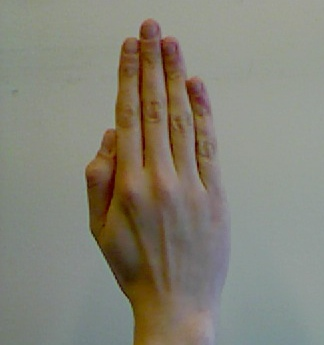
\includegraphics[width=0.2\linewidth,height=0.15\linewidth]{figures/examples/26.jpg}}
\hspace{0.03\linewidth}
\subfloat[Extra4]{\label{fig:hand_27}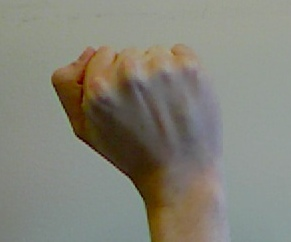
\includegraphics[width=0.2\linewidth,height=0.15\linewidth]{figures/examples/27.jpg}}
\end{center}
\caption{The extra hand poses}
\label{fig:hands_extra}
\end{figure}


\section{Evaluation}
